\section{Case Study} \label{sec:case}
In this section we will conduct one case study to demonstrate how the device-architecture co-optimization methodology can help design STT-RAM cache with different optimization directions. We will replace the L1 SRAM instruction cache and data cache by there different STT-RAM caches: latency-optimized STT-RAM, energy-optimized STT-RAM, or EDP-optimized STT-RAM. Most the optimization techniques are the same with those used to optimize the $64MB$ STT-RAM chip in Section~\ref{subsec:co-opt}. We are the first to explore design space of STT-RAM utilizing PMTJ as L1 cache replacement and compare the results with SRAM.

\subsection{Experimental Setup}
In our simulation, an system-level ARM simulator~\cite{FaCSim} is modified to conduct the evaluation of the latency and energy consumption of the system. As shown in Table.\ref{tb:parameters}, the simulator underlying kernel is SystemC 2.2.0 and it is compatible to ARM9TDMI and XScale architecture. Based on this simulator, we develop a STT-RAM cache module with precise timing and energy model. The 4-way associated  L1 cache in our simulation has the size of 16KB with the cache line size of 32bits. The main memory is implemented with a 64MB embedded DRAM. Besides, we use the MiBench~\cite{MiBench}as the benchmarks for our simulation.

\begin{table}[t]
\centering
\caption{Simulation Parameters}
\label{tb:parameters}
\vspace{-5pt}
\begin{tabular}{ l | c }
\hline \hline
Components & Features\\
\hline
Simulator kernel & SystemC 2.2.0\\
\hline
CPU core & ARM9TDMI and XScale compatible \\
\hline
\multirow{3}{*}{Cache configurations} & 4-way associative 16K L1 data cache \\
& 4-way associative 16K L1 instruction cache \\
& 4B cache line size \\
\hline
\multirow{2}{*}{Bus} & 32-bit address bus  \\
& 32-bit data bus \\
\hline
Clock frequency & $1GHz$ \\
\hline
Main memory & 64MB DRAM \\
\hline
Benchmark & MiBench \\
\hline\hline
\end{tabular}
\vspace{-10pt}
\end{table}

\subsection{Experimental Results}

\begin{figure}[t]
\centering
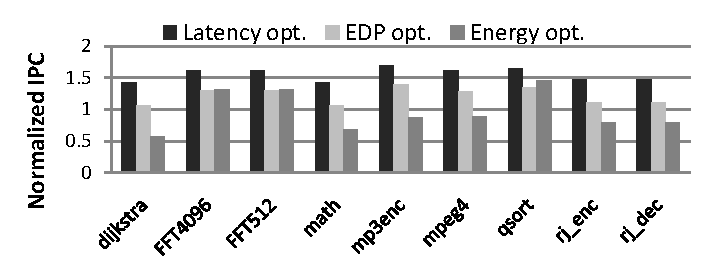
\includegraphics[width=0.4\textwidth]{fig/IPC}
\vspace{-10pt}
\caption{Normalized IPC for STT-RAM with different optimization directions.}
\label{fig:ipc}
\vspace{7pt}
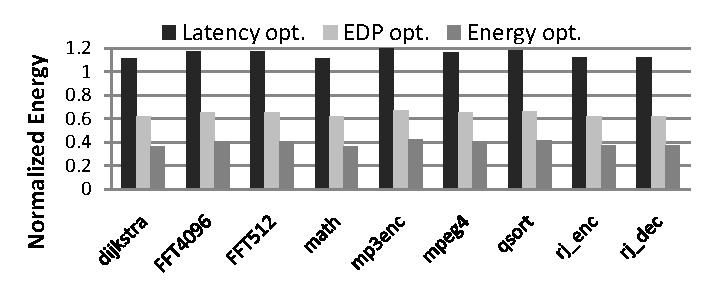
\includegraphics[width=0.4\textwidth]{fig/Energy}
\vspace{-10pt}
\caption{Normalized energy for STT-RAM with different optimization directions.}
\label{fig:energy}
\vspace{7pt}
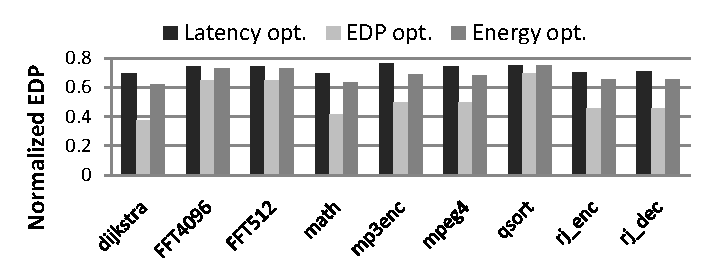
\includegraphics[width=0.4\textwidth]{fig/EDP}
\vspace{-10pt}
\caption{Normalized EDP for STT-RAM with different optimization directions.}
\label{fig:edp}
\vspace{-10pt}
\end{figure}

\begin{figure}[t]
  \centering
  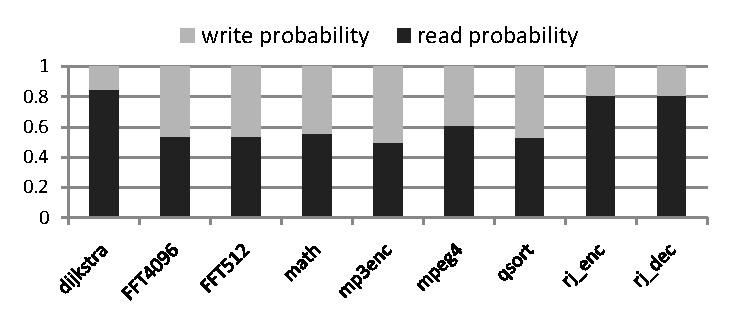
\includegraphics[width=2.8in]{fig/RWratio.eps}
%  \vspace{-10pt}
  \caption{Read-write ratio for different benchmarks.}
  \label{fig:ratio}
\vspace{-15pt}
\end{figure}

We normalize instruction per cycle (IPC), energy and EDP to SRAM-based cache. Note that energy here includes read dynamic energy, write dynamic energy and leakage energy. Fig.~\ref{fig:ipc} shows the simulations results in terms of normalized IPC when using the three different STT-RAM caches. Fig.~\ref{fig:energy} presents the energy saving percentage of replacing SRAM by these STT-RAM caches. Fig.~\ref{fig:edp} illustrates the EDP value of STT-RAM caches for different benchmarks. We can see that the latency-optimized STT-RAM has almost 50\% better IPC than SRAM, while it has negative energy saving compared to SRAM. Energy-optimized STT-RAM has approximately 60\% average energy saving compared to SRAM while IPC is 8\% degraded than SRAM. EDP-optimized STT-RAM has about 20\% better IPC than SRAM and also nearly 40\% energy saving compared to SRAM. Fig.~\ref{fig:ratio} shows the variation in read/write statistics for different benchmarks. 